\section{Introduction}

Vector field analysis is a cornerstone of scientific visualization, providing critical insights into systems that involve particle interactions such as aerodynamics and fluid dynamic modeling, and areas that exhibit consistent forces such as gravitational modeling and magnetic fields.

These fields consist of a grid of discretely spaced points that are each assigned a vector.
This vector serves to store the strength and direction of motion around that point at a given instance.

To be able to effectively understand and analyze these fields, researchers rely on various models of these fields to identify key attributes such as vorticity, divergence, critical points, and flux.


\subsection{Streamline Analysis}

A streamline represents the path that an object would take if it moved through a static vector field. The path is traced by starting from a given vector and always proceeding in the direction of the current vector iteratively.
By connecting these directions throughout the field, streamlines illustrate how a substance or particle would flow at a particular instant.
This approach provides valuable insight into the topology of a given vector field.
This allows researchers to easily identify the overarching flow of a field, its sources and sinks, and other points of criticality.

Formally, a streamline is a curve that follows the direction of the vector field at every point, representing the path an object would take if it moved through the field at a given instant. For a steady vector field $\mathbf{v}(\mathbf{x})$, a streamline $\mathbf{x}(s)$ is defined by the differential equation:
\begin{equation}
	\frac{d\mathbf{x}}{ds} = \mathbf{v}(\mathbf{x}(s))
\end{equation}
where $s$ is a parameter along the curve.

These differ from pathlines, which seek to track a particle's progress over time.
In comparison, streamlines allow for a more comprehensive snapshot of entire vector fields at a static level; they can also be used to show how a given field changes over time, which is highly relevant to disciplines like magnetism.
This broader reach leads to a far higher complexity for streamline tracing in comparison to pathlines.


\begin{figure}[htbp]
	\centering
	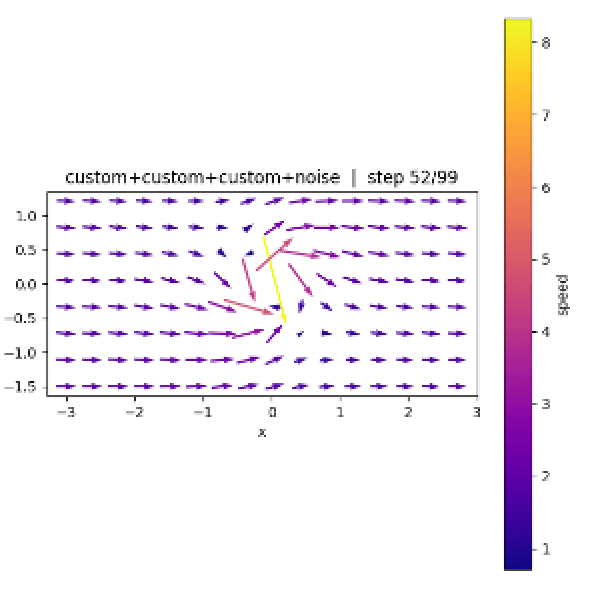
\includegraphics[width=0.8\linewidth]{media/vector-field.png}
	\caption{A discrete vector field grid representing force and direction at each point.}
	\label{fig:vector_field_grid}
\end{figure}

\begin{figure}[htbp]
	\centering
	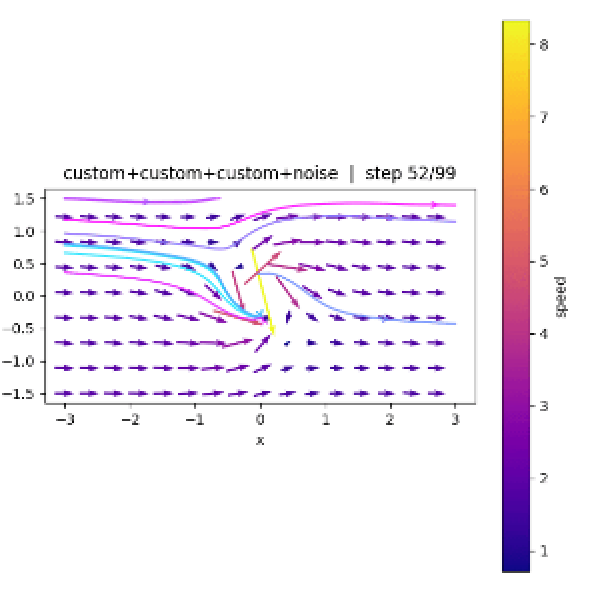
\includegraphics[width=0.8\linewidth]{media/vector-streams.png}
	\caption{A vector field grid with high-velocity streamlines highlighted to illustrate flow patterns.}
	\label{fig:vector_streams_highlighted}
\end{figure}


\subsection{Computational Challenges}

Despite their utility, streamline visualization faces significant computational overhead.

When analyzing large-scale datasets, such as those generated by high-fidelity simulations or astrophysical models, the computational cost of seeding and tracing thousands of streamlines becomes a bottleneck.

A major challenge arises from the irregular memory access patterns inherent in following a path through a grid.
Modern systems utilize caching to help ease the computational slowdown inherent to high I/O operations.
As streamlines are traced, vector points frequently point to subsequent vectors that fall outside of contiguous memory.
This leads to inefficient use of the cache and increased memory latency, which can significantly degrade performance on modern cache-hierarchical architectures.

The joining process of streamlines themselves also introduces challenges as it requires a store of information for each streamline that must be communicated globally to ensure that streamlines are treated as a continuous series.


Additionally, parallel implementations rely heavily on partitioning the dataset into smaller subdomains that can be processed independently.
Due to the inherent out-of-bounds access of vectors, parallel processes are forced to communicate across processes.
This introduces significant communication overhead.
This is especially apparent in GPU-accelerated and distributed implementations where data must be communicated and synchronized between processing units that don't have direct access to the isolated memory of other processes.

Together, these factors make efficient and scalable streamline computation a challenging problem in high-performance vector field analysis.


\subsection{Contributions}

This paper presents a research tool developed in C++17 for the accelerated analysis of 2D vector fields.

We address the computational bottleneck of streamline tracing by implementing and evaluating several parallel computing strategies.

Our primary contributions include:
\begin{itemize}
	\item A modular simulator for generating procedural vector fields (vortices, noise, and custom expressions) stored in HDF5 format.
	\item A suite of parallel analyzer implementations, ranging from shared-memory models (Pthreads, OpenMP) to distributed-memory (OpenMPI) and massively parallel GPU acceleration (CUDA).
	\item A comparative performance study demonstrating the scalability and speedup of these implementations across various field resolutions and streamline densities.
\end{itemize}
